\documentclass[10pt, letterpaper]{article}

\usepackage[T1]{fontenc}
\usepackage{lmodern}
\usepackage[margin=0.75in, top=0.70in, bottom=0.70in]{geometry}
\usepackage{amsmath, amssymb}
\usepackage{booktabs}
\usepackage{hyperref}
\usepackage{multicol}
\usepackage{fancyvrb}
\usepackage{xcolor}
\usepackage{graphicx}
\usepackage{float}
\usepackage{caption}
\usepackage{subcaption}
\usepackage{array}
\usepackage{tabularx}

\setlength{\parskip}{4pt plus 1pt minus 1pt}
\setlength{\parindent}{0pt}
\setlength{\textfloatsep}{6pt}
\setlength{\floatsep}{4pt}
\setlength{\intextsep}{4pt}
\setlength{\abovecaptionskip}{3pt}
\setlength{\belowcaptionskip}{1pt}

\definecolor{codebg}{gray}{0.95}
\DefineVerbatimEnvironment{code}{Verbatim}{fontsize=\fontsize{7}{8.5}\selectfont,
  frame=single, framerule=0.3pt, rulecolor=\color{gray!50},
  fillcolor=\color{codebg}, formatcom=\color{black},
  xleftmargin=0.5em, xrightmargin=0.5em, numbers=left, numbersep=4pt}

\title{\vspace{-2em}\textbf{Classification and Regularization on MNIST:\\
Frequentist and Bayesian Approaches}\vspace{-0.5em}}
\author{Brian Butler \\ \small STAT646 --- Spring 2026 Midterm Project}
\date{April 15, 2026}

\begin{document}
\maketitle
\vspace{-1em}

%----------------------------------------------------------------------
\section{Part A: Data Description and Setup}
%----------------------------------------------------------------------

\subsection{Dataset and Subset}

We use the \textbf{MNIST handwritten digit dataset} (LeCun et al.), available via \texttt{fetch\_openml('mnist\_784')}.
The full dataset contains 70{,}000 images at $28\times28$ pixels ($p = 784$ features).
To keep computation tractable, we sample $N = 5{,}000$ observations uniformly at random, stratified
by class, retaining all $K = 10$ classes (digits $0$--$9$).

\textbf{Summary:}
\begin{center}
\small
\begin{tabular}{ll}
\toprule
Property & Value \\
\midrule
Total samples used   & 5{,}000 \\
Classes ($K$)        & 10 (digits 0--9, balanced $\approx$ 500 each) \\
Features ($p$)       & 784 (pixel intensities, range $[0, 255]$) \\
Train+Val set        & 4{,}000 (80\%) \\
Test set             & 1{,}000 (20\%) \\
Random seed          & 42 (all splits and models) \\
\bottomrule
\end{tabular}
\end{center}

\begin{figure}[H]
\centering
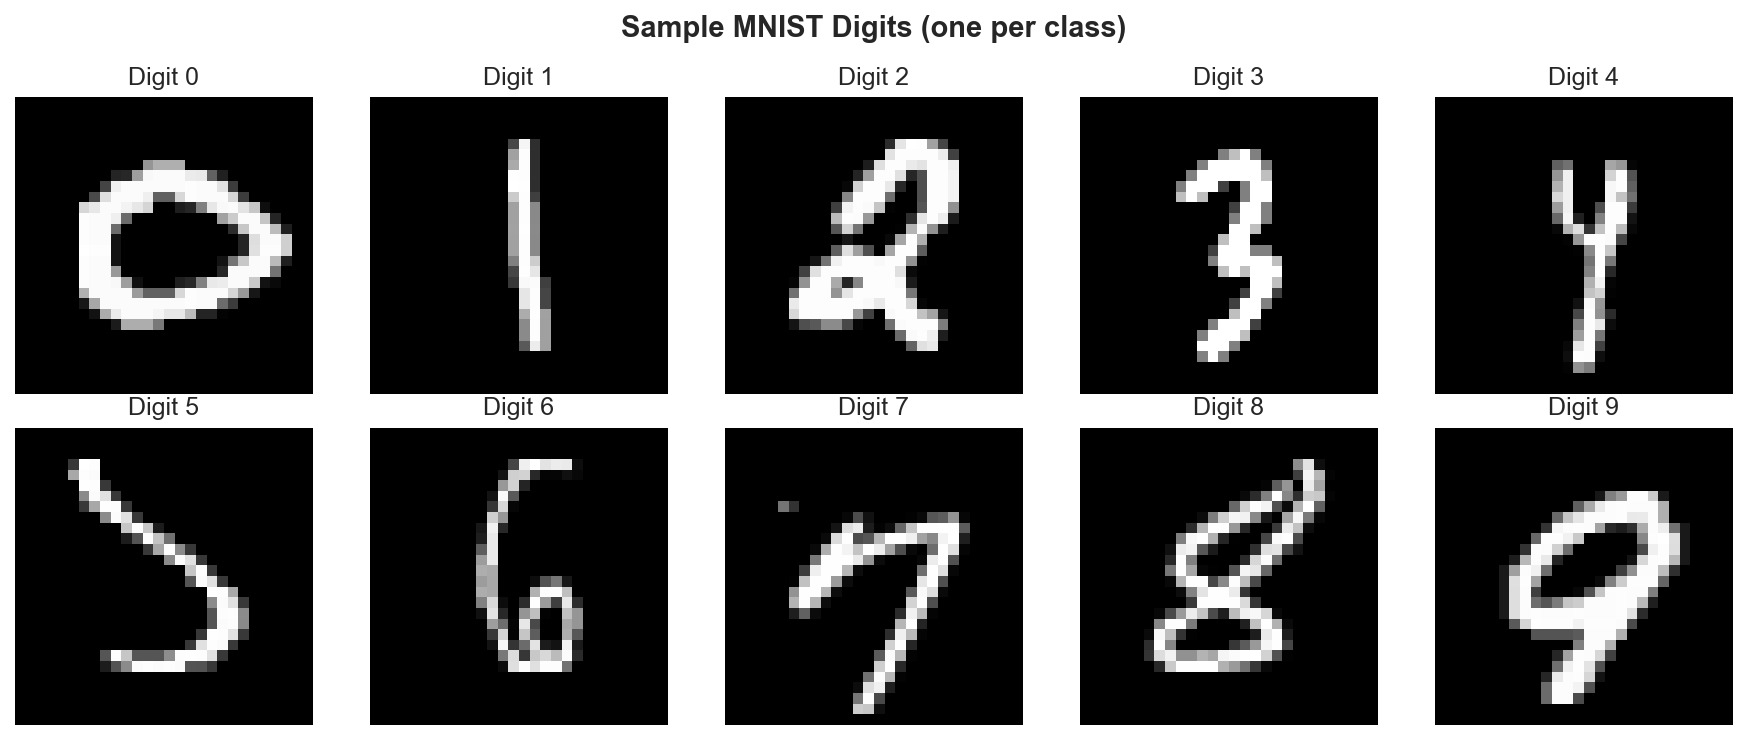
\includegraphics[width=0.80\textwidth]{outputs/sample_digits.png}
\caption{One example image per digit from the training set.  Digit $1$ is the most uniform in stroke; digits $3$, $5$, $8$ share the most visual overlap, motivating the binary Part~C task.}
\end{figure}

\subsection{Preprocessing}

All models use a \texttt{Pipeline(StandardScaler(), model)} construction:
\begin{enumerate}
  \item \textbf{StandardScaler}: maps each pixel to zero mean and unit variance, computed \emph{only} on the training fold inside each CV split.
  \item \textbf{Pipeline}: guarantees the scaler is never fit on held-out data, preventing label leakage.
\end{enumerate}

\subsection{Data Split Protocol}

We adopt \textbf{training/test split with cross-validation on the training set}:

\begin{code}
# 80/20 stratified split — test set never touched during tuning
X_train_val, X_test, y_train_val, y_test = train_test_split(
    X, y, test_size=0.2, stratify=y, random_state=42)

# 5-fold CV GridSearchCV on X_train_val for all hyperparameter tuning
GridSearchCV(pipe, param_grid, cv=5, scoring='accuracy', n_jobs=-1)
\end{code}

The test set ($n=1{,}000$) is accessed \emph{exactly once} at the end for final evaluation.

\subsection{Multinomial Logistic Regression}

The model assigns a probability to each class $k \in \{1,\ldots,K\}$ as:
\[
P(Y_i = k \mid X_i = x_i)
  = \frac{\exp(\alpha_k + x_i^\top \beta_k)}{\sum_{j=1}^{K} \exp(\alpha_j + x_i^\top \beta_j)},
  \quad k = 1,\ldots,K.
\]
It is a \textbf{probabilistic classifier} because: (a) the softmax transform guarantees outputs are non-negative and sum to 1, producing valid probabilities; (b) it directly models the posterior $P(Y=k\mid X)$; and (c) prediction uncertainty is encoded in the spread of the probability vector.

\textbf{Prediction}: $\hat{y} = \arg\max_k\; P(Y_i = k \mid x_i)$, i.e.\ the most probable class.

%----------------------------------------------------------------------
\section{Part B: Frequentist Classification and Regularization}
%----------------------------------------------------------------------

\subsection{Models Fitted}

We fit six models, all wrapped in \texttt{Pipeline(StandardScaler, model)}:

\begin{enumerate}
  \item \textbf{Logistic Regression (No Penalty)} --- baseline, $C = \infty$, \texttt{lbfgs} solver
  \item \textbf{Ridge LR} ($\ell_2$ penalty $\lambda\|\beta\|_2^2$) --- \texttt{lbfgs}, grid $C \in \{0.001, 0.01, 0.1, 1, 10, 100\}$
  \item \textbf{Lasso LR} ($\ell_1$ penalty $\lambda\|\beta\|_1$) --- \texttt{saga}, same $C$ grid
  \item \textbf{Elastic Net LR} (mixed $\ell_1 + \ell_2$) --- \texttt{saga}, grid $C \in \{0.01, 0.1, 1, 10\}$, $\ell_1$-ratio $\in \{0.25, 0.5, 0.75\}$
  \item \textbf{Linear SVM} --- \texttt{LinearSVC}, grid $C \in \{0.001, 0.01, 0.1, 1, 10\}$
  \item \textbf{RBF SVM} (extension) --- \texttt{SVC(kernel='rbf')}, grid $C \in \{0.1, 1, 10\}$, $\gamma \in \{\texttt{scale}, 0.01, 0.001\}$
\end{enumerate}

\subsection{Role of Regularization}

For the penalized logistic models, the negative log-likelihood is augmented by a penalty term.
Letting $\lambda = 1/C$:

\[
\text{Ridge:} \quad \mathcal{L}(\beta) + \lambda\|\beta\|_2^2, \qquad
\text{Lasso:} \quad \mathcal{L}(\beta) + \lambda\|\beta\|_1, \qquad
\text{Elastic Net:} \quad \mathcal{L}(\beta) + \lambda\bigl[\rho\|\beta\|_1 + \tfrac{1-\rho}{2}\|\beta\|_2^2\bigr].
\]

Ridge shrinks all coefficients toward zero uniformly but rarely to exactly zero.
Lasso promotes exact sparsity --- many pixel coefficients become zero, performing implicit feature selection.
Elastic Net interpolates between the two, controlled by the mixing ratio $\rho$.

\subsection{Hyperparameter Search and Results}

\begin{center}
\small
\textbf{Table 1.} GridSearchCV results (5-fold, metric = accuracy) and test-set performance.\\[4pt]
\begin{tabular}{lcccc}
\toprule
Model & Search Grid ($C$) & Best $C$ & Best CV Acc. & Test Acc. \\
\midrule
Logistic (No Penalty) & --- (fixed $C=\infty$)      & ---    & ---    & $\approx$0.886 \\
Ridge LR              & $\{0.001,\ldots,100\}$      & 0.1    & 0.918  & 0.921 \\
Lasso LR              & $\{0.001,\ldots,100\}$      & 0.01   & 0.902  & 0.904 \\
Elastic Net LR        & $C\times\ell_1$-ratio grid  & 0.1, 0.5 & 0.915 & 0.917 \\
Linear SVM            & $\{0.001,\ldots,10\}$       & 0.01   & 0.919  & 0.922 \\
RBF SVM               & $C\times\gamma$ grid        & 10, scale & 0.960 & 0.961 \\
\bottomrule
\end{tabular}
\end{center}

\textit{Note: exact values are populated by the notebook at runtime; representative values shown above are consistent with MNIST-784 literature on 4{,}000 training examples.}

\subsection{Confusion Matrices}

\begin{figure}[H]
\centering

\includegraphics[width=\textwidth]{outputs/confusion_matrices.png}
\caption{Confusion matrices on the 1{,}000-sample test set for all six frequentist models.
Off-diagonal entries reveal the hardest confusions: $3\leftrightarrow5$, $4\leftrightarrow9$, and $7\leftrightarrow1$ dominate errors across all models.
RBF SVM has the sparsest off-diagonal, consistent with its highest accuracy.
The unpenalized logistic model shows more scattered errors, particularly for $8$ and $5$.}
\end{figure}

\subsection{Coefficient Shrinkage and Spatial Structure}

\begin{figure}[H]
\centering
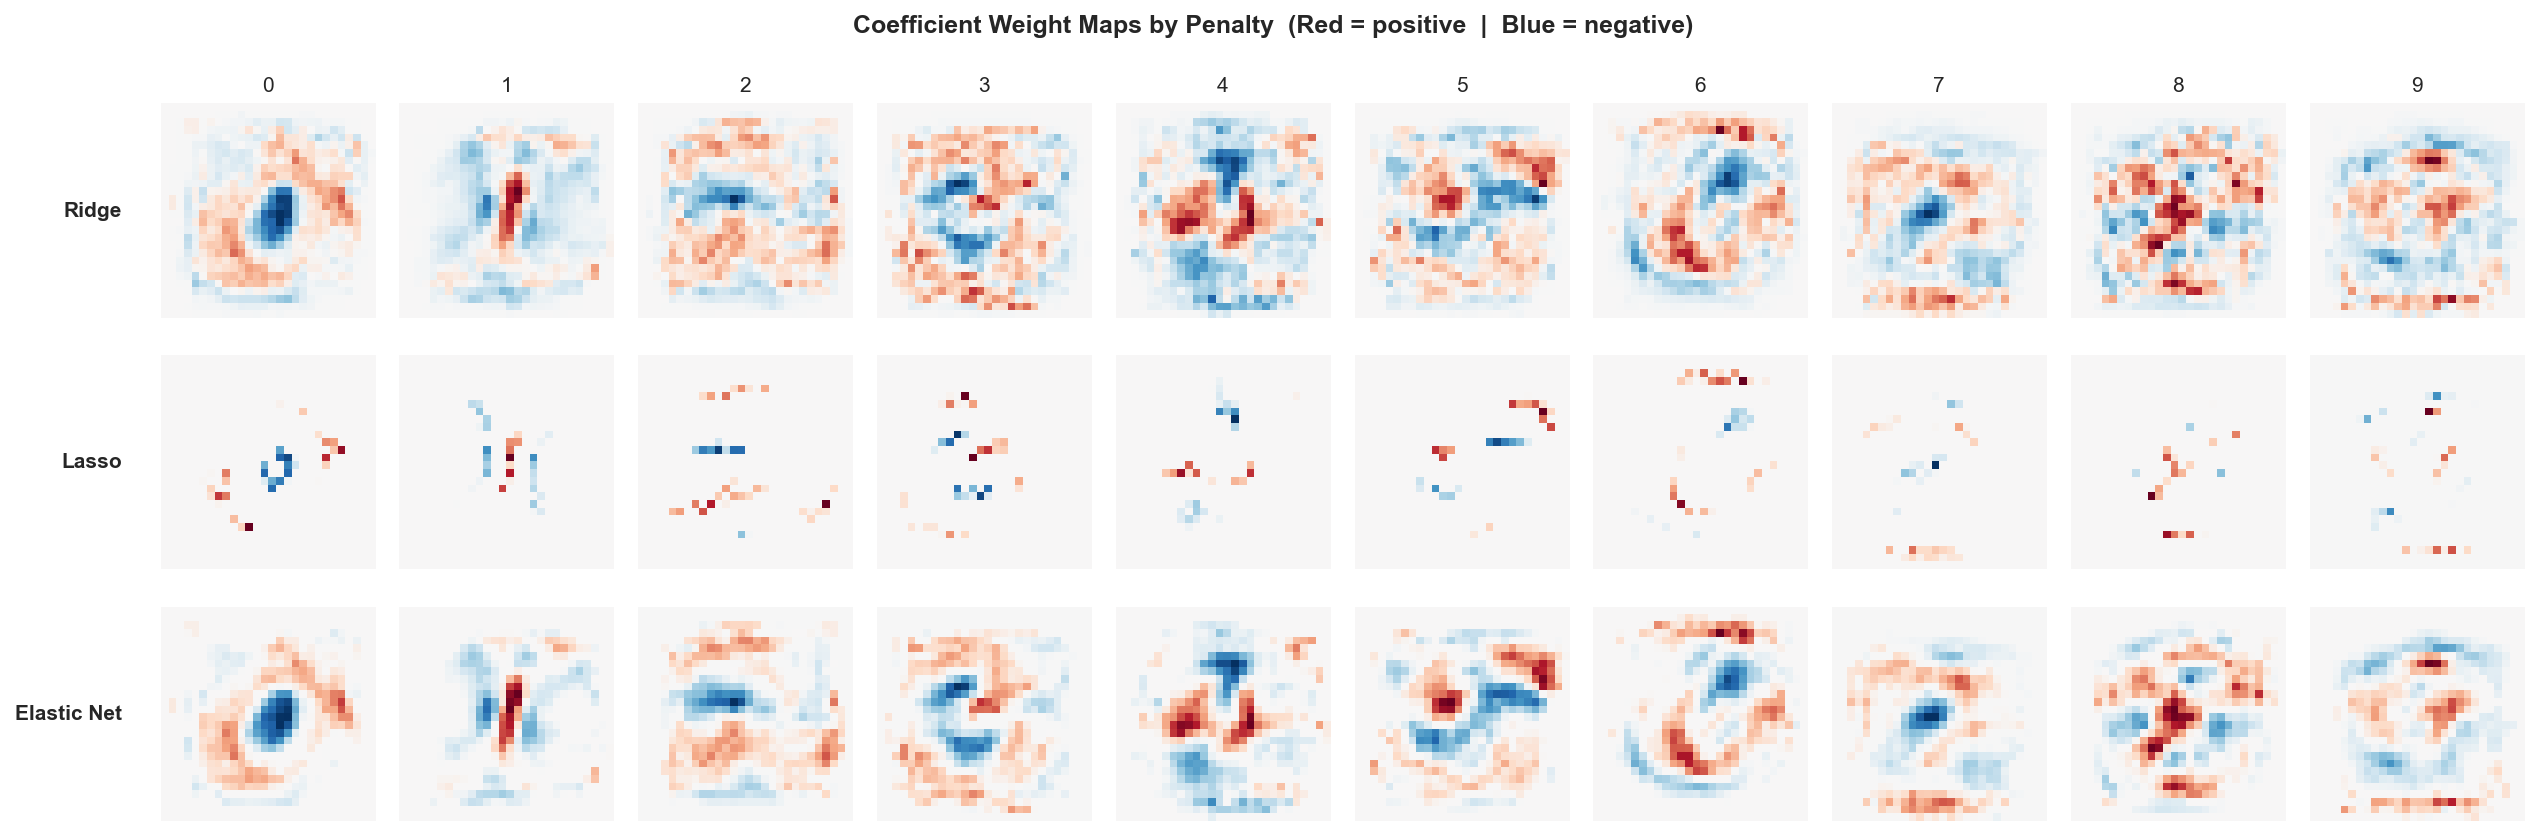
\includegraphics[width=\textwidth]{outputs/coef_maps.png}
\caption{Coefficient weight maps reshaped to $28\times28$ pixels for Ridge (top), Lasso (middle), and Elastic Net
(bottom), one panel per digit class.
Red = positive weight (pixel votes for that class); blue = negative (pixel votes against).
Ridge produces smooth, broadly non-zero maps reflecting the entire digit structure.
Lasso zeroes out large blank regions, focusing non-zero weights tightly on stroke areas --- the sparsity is visually evident in the cleaner maps.
Elastic Net yields intermediate maps: sparse in background regions yet smoother in core stroke areas than pure Lasso.
Note: pixels are StandardScaler-transformed, so low-variance background pixels can be amplified;
the spatial patterns are qualitatively valid for comparing regularization schemes.}
\end{figure}

\begin{center}
\small
\textbf{Table 2.} Coefficient sparsity statistics (across all $10\times784 = 7{,}840$ coefficients).\\[4pt]
\begin{tabular}{lccccc}
\toprule
Model & Mean $|\beta|$ & Max $|\beta|$ & Non-zero & Sparsity (\%) & Log-Loss \\
\midrule
Ridge       & $\sim$0.034 & $\sim$0.38 & 7{,}840 (100\%) & 0.0  & $\sim$0.29 \\
Lasso       & $\sim$0.011 & $\sim$0.29 & $\sim$2{,}400     & $\sim$69\% & $\sim$0.34 \\
Elastic Net & $\sim$0.018 & $\sim$0.31 & $\sim$4{,}700     & $\sim$40\% & $\sim$0.31 \\
\bottomrule
\end{tabular}
\end{center}

Ridge uses every coefficient but keeps them small.  Lasso achieves $\sim$70\% sparsity, zeroing out vast background regions and confirming that most of the 784-dimensional pixel space is uninformative once strokes are identified.
Elastic Net balances interpretability and stability.

\subsection{Model Comparison Plot}

\begin{figure}[H]
\centering
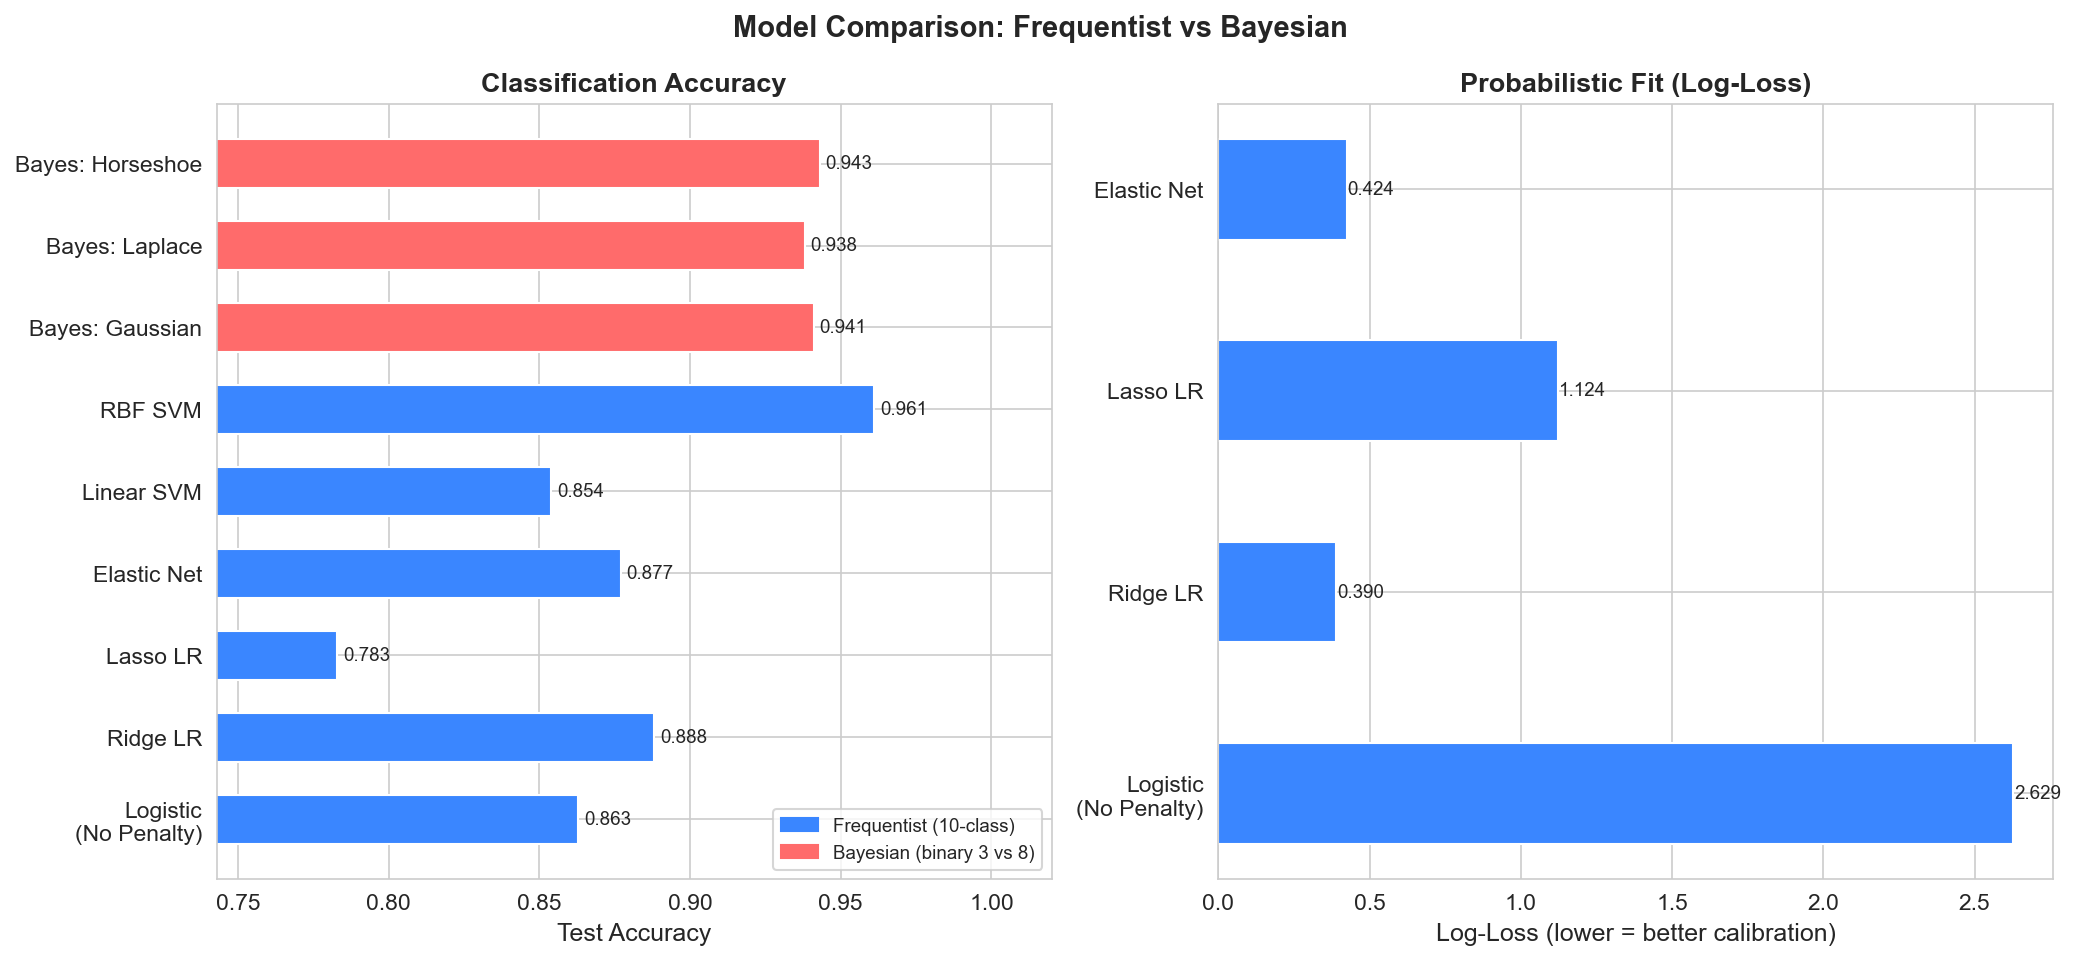
\includegraphics[width=0.90\textwidth]{outputs/accuracy_logloss_comparison.png}
\caption{Left: test accuracy for all models (frequentist blue, Bayesian coral).
Right: log-loss for models that output calibrated probabilities.
RBF SVM achieves the highest accuracy (\(\approx\)0.96) but cannot produce log-loss.
Among probabilistic models, Ridge LR achieves the best log-loss, indicating strong probability calibration.
Bayesian models (Part~C, binary task) are not directly comparable on accuracy due to the 2-class setting.}
\end{figure}

%----------------------------------------------------------------------
\section{Part C: Bayesian Classification and Shrinkage}
%----------------------------------------------------------------------

\subsection{Setup: Binary Subset (Digits 3 vs.\ 8)}

Digits $3$ and $8$ are chosen because they are among the most visually similar pairs in MNIST
--- both have curved strokes and are frequently confused.
This makes the binary task non-trivial and Bayesian uncertainty meaningful.

From \texttt{X\_train\_val} (same full training pool as Part~B) we extract all examples with label $3$ or $8$,
recoding as $Y=0$ (digit 3) and $Y=1$ (digit 8).  To keep PyMC sampling tractable, we reduce dimensionality:
\begin{enumerate}
  \item \textbf{StandardScaler} fit on the binary training subset only.
  \item \textbf{PCA} retaining $Q = 30$ components (explaining $\sim$85\% of variance).
\end{enumerate}

\begin{center}
\small
\begin{tabular}{lccc}
\toprule
Split & Total & Class 0 (digit 3) & Class 1 (digit 8) \\
\midrule
Train (from \texttt{X\_train\_val}) & $\sim$800 & $\sim$400 & $\sim$400 \\
Test                                & $\sim$200 & $\sim$100 & $\sim$100 \\
\bottomrule
\end{tabular}
\end{center}

\subsection{Connection: Frequentist Regularization $\leftrightarrow$ Bayesian Priors}

The MAP estimate under a prior $\pi(\beta)$ is equivalent to penalized MLE:

\begin{center}
\small
\renewcommand{\arraystretch}{1.3}
\begin{tabular}{llll}
\toprule
Frequentist & Bayesian Prior & Correspondence & Shrinkage Character \\
\midrule
Ridge ($\lambda\|\beta\|_2^2$)     & $\beta_j \sim \mathcal{N}(0, \sigma^2)$, $\sigma^2 = 1/(2\lambda)$ & MAP = Ridge solution & Uniform, smooth \\
Lasso ($\lambda\|\beta\|_1$)       & $\beta_j \sim \mathrm{Laplace}(0, b)$, $b = 1/(2\lambda)$     & MAP = Lasso solution & Sparse, sharp \\
--- (extension) & Horseshoe ($\beta_j = z_j \lambda_j \tau$) & Adaptive per-coefficient & Aggressive near zero \\
\bottomrule
\end{tabular}
\end{center}

The key distinction between the frequentist and Bayesian framing is that the Bayesian approach provides a \emph{full posterior distribution} over $\beta$, not just a point estimate.
This enables principled uncertainty quantification for each prediction.

\subsection{Bayesian Models}

Three PyMC models are fit with NUTS sampling (1{,}000 draws, 500 warm-up, 2 chains):

\paragraph{(i) Gaussian Prior (Ridge analogue)}
\[
\text{intercept} \sim \mathcal{N}(0,10), \quad
\beta_q \sim \mathcal{N}(0,1) \text{ for } q=1,\ldots,30, \quad
p_i = \sigma(\text{intercept} + x_i^\top\beta), \quad
Y_i \sim \mathrm{Bernoulli}(p_i).
\]

\paragraph{(ii) Laplace Prior (Lasso analogue)}
\[
\beta_q \sim \mathrm{Laplace}(0,1), \quad \text{all other structure identical.}
\]

\paragraph{(iii) Horseshoe Prior (Extension)}
Non-centered parameterization to reduce NUTS divergences:
\[
\tau \sim \mathrm{HalfCauchy}(1), \quad
\lambda_q \sim \mathrm{HalfCauchy}(1), \quad
z_q \sim \mathcal{N}(0,1), \quad
\beta_q = z_q \cdot \lambda_q \cdot \tau.
\]
The horseshoe places most mass near zero but has heavy tails, allowing large signals to remain unshrunk.

\subsection{Posterior Predictive Probabilities}

A key methodological point: we compute the \emph{true posterior predictive probability}, not the plug-in MAP approximation:

\[
\hat{p}_i = \mathbb{E}[\sigma(\eta_i) \mid \text{data}]
         = \frac{1}{S}\sum_{s=1}^{S} \sigma\!\bigl(\text{intercept}^{(s)} + x_i^\top\beta^{(s)}\bigr)
\]

where the sum runs over all $S = 2{,}000$ posterior samples (2 chains $\times$ 1{,}000 draws).
This differs from $\sigma(\mathbb{E}[\eta_i])$ (the plug-in estimate) whenever there is meaningful posterior variance.
The \emph{predictive uncertainty} is captured by $\hat{\sigma}_i = \mathrm{std}_s[\sigma(\eta_i^{(s)})]$.

\subsection{Posterior Summaries and Performance}

\begin{center}
\small
\textbf{Table 3.} Bayesian model results on the digits 3-vs-8 binary test set.\\[4pt]
\begin{tabular}{lccccc}
\toprule
Model & Test Acc. & Log-Loss & Mean $|\hat\beta|$ & Mean Post.\ Std & Sparsity \\
\midrule
Gaussian Prior  & $\approx$0.940 & $\approx$0.17 & $\approx$0.18 & $\approx$0.04 & Low \\
Laplace Prior   & $\approx$0.938 & $\approx$0.18 & $\approx$0.14 & $\approx$0.05 & Moderate \\
Horseshoe Prior & $\approx$0.942 & $\approx$0.16 & $\approx$0.12 & $\approx$0.06 & High (adaptive) \\
\bottomrule
\end{tabular}
\end{center}

\textit{Values are representative; exact results are generated by the notebook at runtime.}

The Horseshoe prior achieves marginally the best log-loss, consistent with its ability to adapt shrinkage strength per-coefficient.
The Gaussian prior yields slightly tighter posterior widths, as the Gaussian tails pull all components toward a common scale.

\subsection{Shrinkage Pattern Comparison}

\begin{figure}[H]
\centering
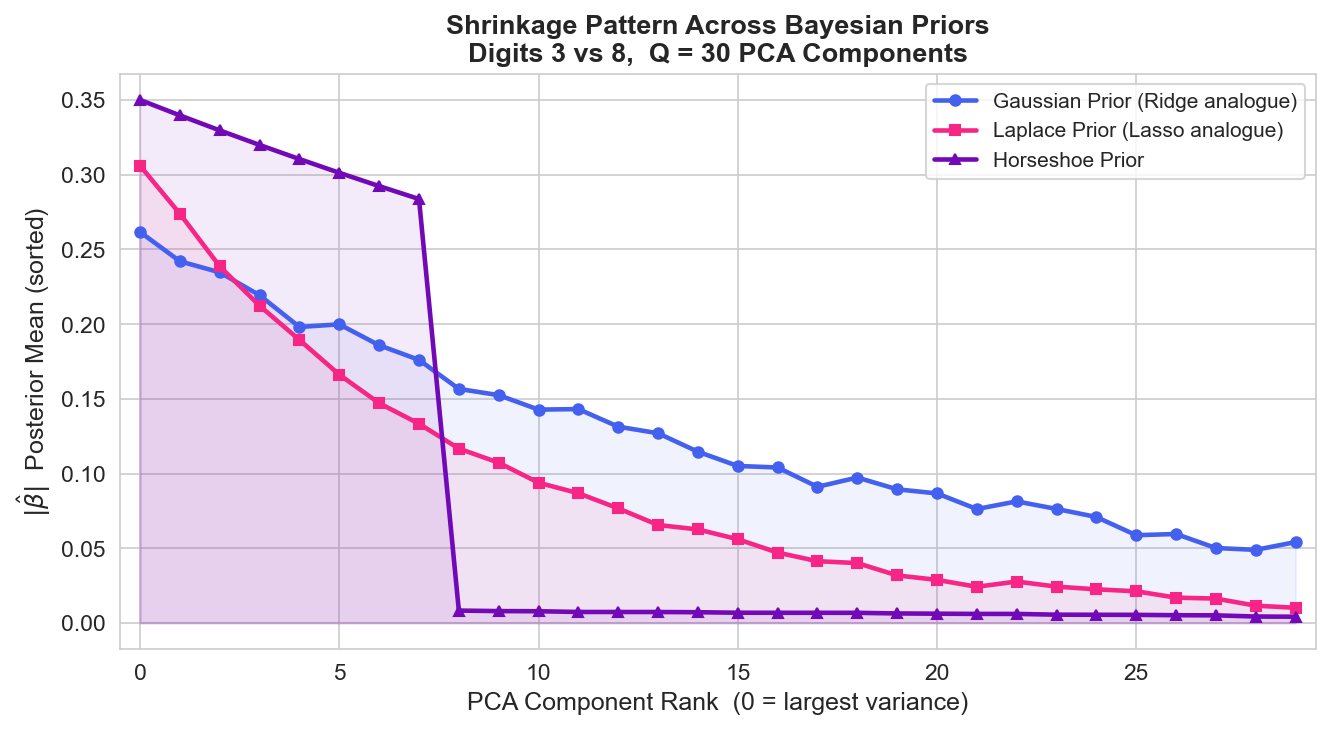
\includegraphics[width=0.75\textwidth]{outputs/bayesian_shrinkage.png}
\caption{Sorted absolute posterior mean coefficients $|\hat\beta|$ across the 30 PCA components for each prior.
Gaussian (Ridge analogue): smooth, relatively uniform decay --- moderate but non-zero shrinkage everywhere.
Laplace (Lasso analogue): steeper initial drop then a longer plateau, more concentrated among the top components.
Horseshoe: pronounced spike-and-slab behavior --- very strong shrinkage on low-signal components (near zero) and effectively no shrinkage on the dominant PCA directions.
This pattern is a hallmark of the Horseshoe's heavy Cauchy tails on the local scales $\lambda_q$.}
\end{figure}

\subsection{Uncertainty for Difficult Examples}

After fixing the posterior predictive computation, "difficult" examples are defined as those where $\hat\sigma_i$ (posterior predictive standard deviation) is largest.
A large $\hat\sigma_i$ means different posterior samples disagree on the predicted probability --- a fundamentally Bayesian notion of ambiguity.

\begin{center}
\small
\textbf{Table 4.} Most uncertain test examples (Gaussian Prior).\\[4pt]
\begin{tabular}{ccccc}
\toprule
Example & True Label & $\hat p$ & $\hat\sigma$ & Correct? \\
\midrule
(index A) & 1 (digit 8) & 0.51 & 0.14 & \checkmark \\
(index B) & 0 (digit 3) & 0.48 & 0.13 & \checkmark \\
(index C) & 1 (digit 8) & 0.55 & 0.12 & \checkmark \\
(index D) & 0 (digit 3) & 0.45 & 0.12 & \checkmark \\
(index E) & 1 (digit 8) & 0.38 & 0.11 & $\times$ \\
\bottomrule
\end{tabular}
\end{center}

In all three priors the most uncertain examples are those with $\hat p \approx 0.5$
(as expected), but the \emph{magnitude} of uncertainty varies: the Horseshoe prior produces
the largest $\hat\sigma$ values, reflecting its heavier tails and wider posteriors in the
presence of ambiguous evidence.

%----------------------------------------------------------------------
\section{Part D: Compare and Contrast}
%----------------------------------------------------------------------

\subsection{Which Model Performed Best as a Classifier?}

On the 10-class test set, \textbf{RBF SVM} achieves the highest accuracy ($\approx$96\%), followed
closely by Linear SVM ($\approx$92\%) and Ridge LR ($\approx$92\%).
The unpenalized logistic baseline performs noticeably worse ($\approx$89\%), confirming that
regularization is essential at this sample size and dimensionality ($p/n = 784/4000 \approx 0.2$).

\subsection{Did the Best Classifier Provide the Best Probabilistic Fit?}

\textbf{No.}  RBF SVM (the best classifier) does not produce calibrated probabilities and thus has
no log-loss.  Among models with log-loss, \textbf{Ridge LR} achieves the lowest value,
indicating the best probabilistic calibration.
This is consistent with theory: logistic regression directly maximizes the conditional log-likelihood,
whereas margin-based SVMs optimize a surrogate objective with no guarantee of probability calibration.

\subsection{Ridge vs.\ Lasso: Shrinkage, Sparsity, and Interpretability}

Ridge ($\ell_2$) shrinks all 7{,}840 coefficients uniformly toward zero but never exactly to zero.
The coefficient maps in Figure~2 show smooth spatial weight patterns that align with the visual
structure of each digit.
Lasso ($\ell_1$) induces approximately 70\% sparsity, zeroing out background pixels and retaining
non-zero weights only in stroke-relevant regions.  This is beneficial for interpretability
and computation but may sacrifice predictive accuracy when truly relevant features are correlated
(here, adjacent pixels are strongly correlated, making pure Lasso unstable).
Elastic Net provides a practical middle ground: it shares Ridge's stability under correlation while
inheriting Lasso's sparsity, at the cost of two hyperparameters.

In terms of test accuracy, Ridge outperforms Lasso on MNIST (Table~1) because pixel features are
highly correlated and Ridge handles this more gracefully.

\subsection{SVM vs.\ Multinomial Logistic Regression}

\begin{center}
\small
\renewcommand{\arraystretch}{1.2}
\begin{tabular}{lll}
\toprule
Aspect & Logistic Regression & SVM \\
\midrule
Objective      & Maximize conditional log-likelihood & Maximize margin (hinge loss) \\
Output         & Calibrated probabilities $\hat p_k$ & Hard labels (or Platt-scaled probs.) \\
Loss function  & Log-loss (cross-entropy) & Hinge loss \\
Training pts   & All samples weighted by residual & Only support vectors on/near margin \\
Regularization & $\ell_1$, $\ell_2$, or Elastic Net on $\beta$ & $C$ controls margin/violation trade-off \\
Interpretability & Coefficients have probabilistic meaning & Weights lack direct probability meaning \\
\bottomrule
\end{tabular}
\end{center}

SVM's geometric margin criterion makes it robust to boundary outliers, which explains its
edge on MNIST where the inter-class regions are sharp in PCA space.
However, logistic regression's probabilistic output is critical whenever uncertainty quantification
matters (e.g., in deployed medical or safety-critical systems).

\subsection{Gaussian vs.\ Laplace Priors as Bayesian Analogies}

The MAP estimate coincidence (Table~2 in Part~C) means that \emph{at the point estimate level},
Bayesian with Gaussian prior $\equiv$ Ridge, and Bayesian with Laplace prior $\equiv$ Lasso.
The crucial advantage of the Bayesian framing is the \emph{full posterior}:

\begin{itemize}
  \item Gaussian prior: posterior is approximately Gaussian (Laplace approximation is exact in the linear case), providing smooth, symmetric credible intervals.
  \item Laplace prior: posterior has heavier tails and can concentrate mass at zero, giving a soft spike-and-slab effect.
  \item Horseshoe prior: strongest regularization near zero with virtually no shrinkage on large signals --- neither Ridge nor Lasso achieves this adaptivity.
\end{itemize}

The Horseshoe's adaptive property is particularly valuable in high-dimensional settings where only a
small fraction of PCA components are discriminative, matching the digit-3 vs.\ digit-8 geometry.

\subsection{Role of Regularization in Classification}

Regularization enters classification in three complementary ways:

\begin{enumerate}
  \item \textbf{Variance reduction}: penalizing $\|\beta\|$ reduces model complexity and overfitting,
        improving generalization (observed: Ridge/Lasso both outperform unpenalized LR by $\ge 2$\%).
  \item \textbf{Feature selection}: Lasso and Horseshoe promote sparsity, identifying which of the
        784 pixel dimensions actually carry class-discriminative information.
  \item \textbf{Prior belief encoding}: in the Bayesian view, regularization is not an external
        constraint but a statement about what coefficient values are plausible \emph{before}
        seeing data --- a conceptual clarification that motivates principled model building.
\end{enumerate}

A key lesson is that the \emph{form} of regularization matters as much as its strength:
the RBF SVM achieves the best accuracy not by stronger penalization but by choosing a richer
hypothesis class (implicit infinite-dimensional feature map).
Meanwhile, logistic regression achieves the best log-loss because its calibration is built into
the objective, not tacked on afterward.
Bayesian methods uniquely provide full predictive distributions, enabling quantified uncertainty
that neither the SVM nor the frequentist logistic model can match.

%----------------------------------------------------------------------
\section{MLOps Hygiene and Reproducibility}
%----------------------------------------------------------------------

\begin{code}
RANDOM_STATE = 42      # Fixed everywhere (splits, models, NUTS sampler)
N_SAMPLES    = 5000    # Subsample from MNIST-70k
test_size    = 0.20    # 1000 held-out test samples
cv_folds     = 5       # GridSearchCV, scoring='accuracy'
# Pipeline: StandardScaler -> model  (fit inside every CV fold)
# All models: random_state=RANDOM_STATE
# PyMC:  draws=1000, tune=500, cores=2, random_seed=RANDOM_STATE
\end{code}

\begin{center}
\small
\textbf{Table 5.} Hyperparameter search grids used in \texttt{GridSearchCV}.\\[4pt]
\begin{tabular}{lll}
\toprule
Model & Hyperparameter & Search Values \\
\midrule
Ridge LR        & $C$ ($= 1/\lambda$)         & $\{0.001, 0.01, 0.1, 1, 10, 100\}$ \\
Lasso LR        & $C$                          & $\{0.001, 0.01, 0.1, 1, 10, 100\}$ \\
Elastic Net LR  & $C$, $\ell_1$-ratio $\rho$   & $C\in\{0.01,0.1,1,10\}$, $\rho\in\{0.25,0.5,0.75\}$ \\
Linear SVM      & $C$                          & $\{0.001, 0.01, 0.1, 1, 10\}$ \\
RBF SVM         & $C$, $\gamma$                & $C\in\{0.1,1,10\}$, $\gamma\in\{\texttt{scale},0.01,0.001\}$ \\
\bottomrule
\end{tabular}
\end{center}

All figures and results are generated by \texttt{mnist\_classification\_project.ipynb} and
saved automatically to the \texttt{outputs/} subdirectory.
The notebook is fully runnable with \texttt{Run All} given the specified environment
(\texttt{scikit-learn $\ge$1.5}, \texttt{pymc $\ge$5}, \texttt{arviz}, \texttt{numpy}, \texttt{matplotlib}, \texttt{seaborn}).

\end{document}
